\section{Results}
\label{sec:results}
% Summary of subsections
In this section, we first discuss the experimental platform for data collection and experiments. Second, we discuss the key conceptual reasoning behind our combined method of our meta-learning algorithm, called \DAML,~and our composite adaptive controller with stability guarantees. Third, we discuss several experiments to quantitatively compare the closed-loop trajectory-tracking performance of our methods to \revision{a nonlinear baseline method and two state-of-the-art adaptive flight control methods, and we observe our methods reduce the average tracking error substantially.} In order to demonstrate the new capabilities brought by our methods, we present agile flight results in gusty winds, where the UAV must quickly fly through narrow gates that are only slightly wider than the vehicle. \revision{Finally, we show our methods are also applicable in outdoor agile tracking tasks without external motion capture systems.}

\begin{figure}[htbp]
    \centering
    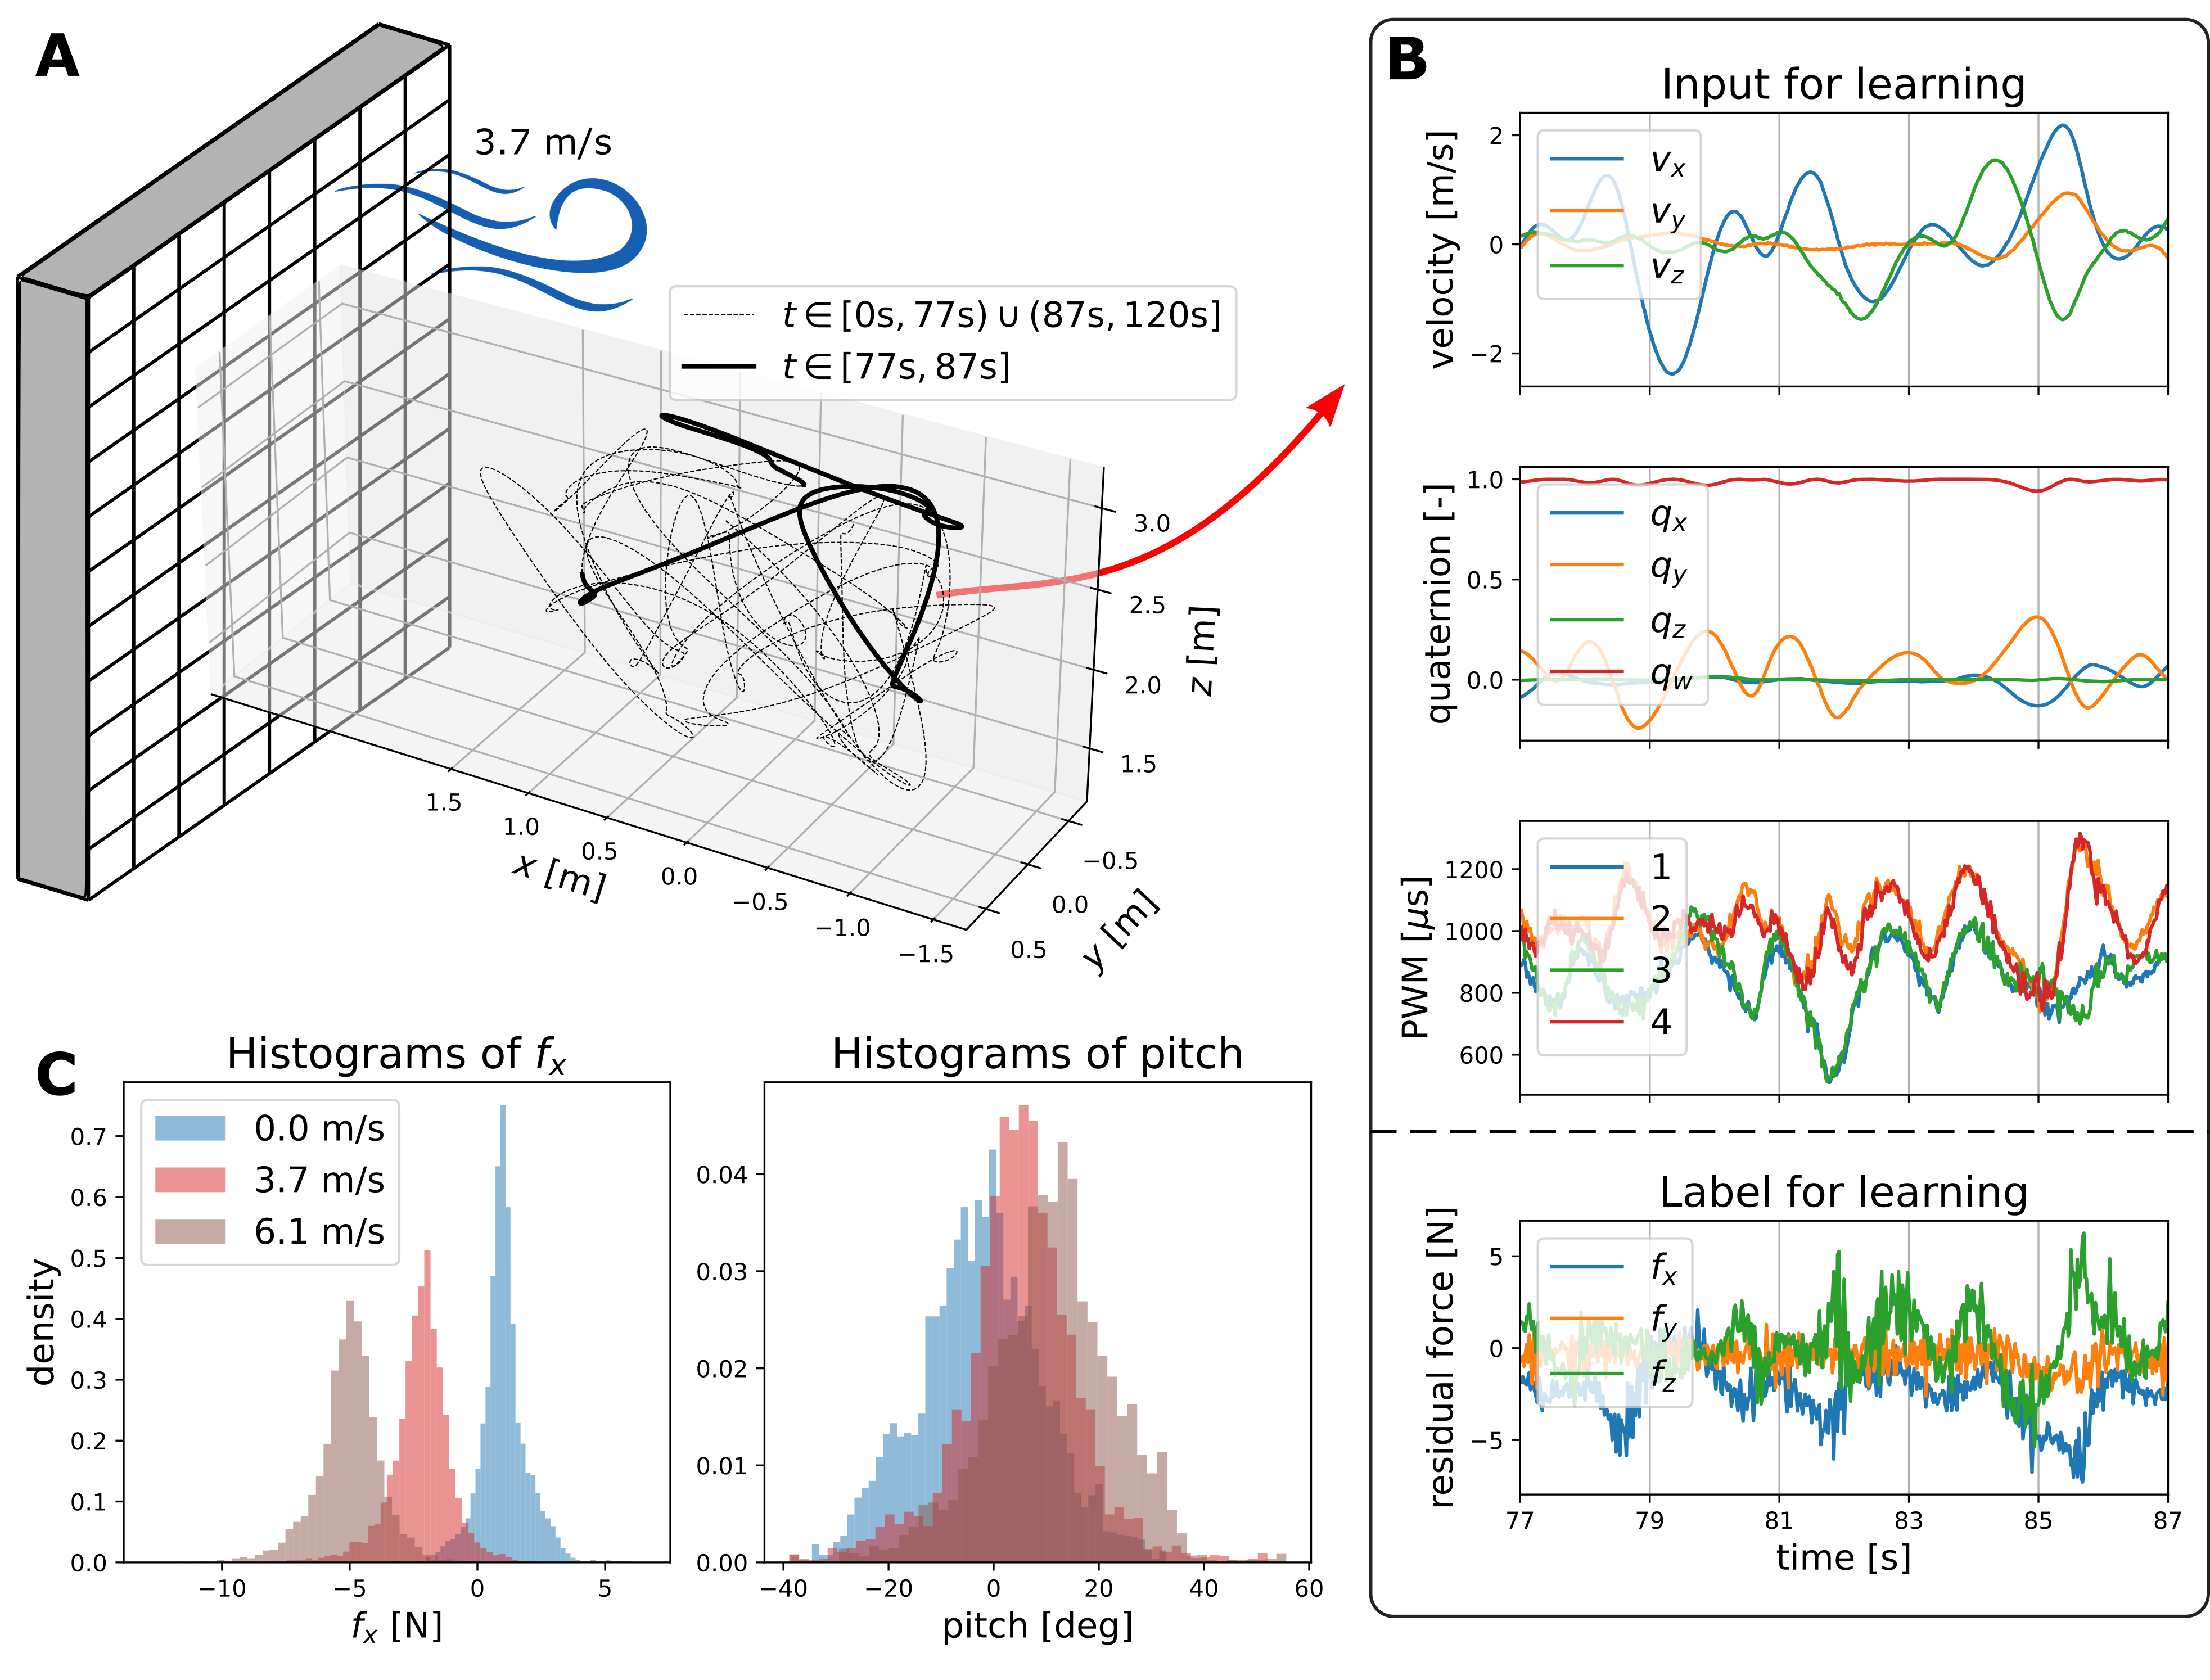
\includegraphics[width=0.8\linewidth]{figures/figure_training_data.png}
    \caption{\textbf{Training data collection.} (\textbf{A}) The xyz position along a two-minute randomized trajectory for data collection with wind speed \SI{8.3}{km/h} (\SI{3.7}{m/s}), in the Caltech Real Weather Wind Tunnel. (\textbf{B}) A typical 10-second trajectory of the inputs (velocity, attitude quaternion, and motor speed PWM command) and label (offline calculation of aerodynamic residual force) for our learning model, corresponding to the highlighted part in (A). (\textbf{C}) Histograms showing data distributions in different wind conditions. (\textbf{C}) \textbf{Left:} distributions of the $x$-component of the wind-effect force, $f_x$. This shows that the aerodynamic effect changes as the wind varies. (\textbf{C}) \textbf{Right:} distributions of the pitch, a component of the state used as an input to the learning model. This shows that the shift in wind conditions causes a distribution shift in the input.}
    \label{fig:training-data}
\end{figure}

\subsection*{Experimental Platform}
% Overview of facilities for experiments
All of our experiments are conducted at Caltech's Center for Autonomous Systems and Technologies (CAST). The experimental setup consists of an OptiTrack motion capture system with \revision{12 infrared} cameras for localization \rev{streaming position measurements at \SI{50}{Hz}}, a WiFi router for communication, the Caltech Real Weather Wind Tunnel
for generating dynamic wind conditions, and a custom-built quadrotor UAV. 
The Real Weather Wind Tunnel is composed of 1296 individually controlled fans and can generate uniform wind speeds of up to \revision{\highwind} in its 3x3x5\SI{}{m} test section. \revision{For outdoor flight, the drone is also equipped with a Global Positioning System (GPS) module and an external antenna.}
We now discuss the design of the UAV and the wind condition in detail.

% Overview of quadrotor platform
\paragraph{UAV Design} We built a quadrotor UAV for our primary data collection and all experiments, shown in \cref{fig:intro}(A).
The quadrotor weighs \revision{\SI{2.6}{kg}} with a thrust to weight ratio of $2.2$. The UAV is equipped with a Pixhawk flight controller running PX4, an open-source commonly used drone autopilot platform \cite{meier_pixhawk_2012}. The UAV incorporates a Raspberry Pi 4 onboard computer running a Linux operation system, which performs real-time computation and adaptive control and interfaces with the flight controller through MAVROS, an open-source set of communication drivers for UAVs. State estimation is performed using the built-in PX4 Extended Kalman Filter (EKF), which fuses inertial measurement unit (IMU) data with global position estimates from OptiTrack motion capture system \revision{(or the GPS module for outdoor flight tasks)}. The UAV platform features a wide-X configuration, measuring \SI{85}{cm} in width, \SI{75}{cm} in length, and \SI{93}{cm} diagonally, and tilted motors for improved yaw authority. \rev{This general hardware setup is standard and similar to many quadrotors.} We refer to the supplementary materials (\ref{sec:supp-drone-configuration}) for further configuration details.

% Overview of software and implementation of controller
We implemented our control algorithm and the baseline control methods in the position control loop in Python, and run it on the onboard Linux computer at \SI{50}{Hz}. The PX4 was set to the offboard flight mode and received thrust and attitude commands from the position control loop. The built-in PX4 multicopter attitude controller was then executed at the default rate, which is a linear PID regulation controller on the quaternion error. The online inference of the learned representation is also in Python via PyTorch, which is an open source deep learning framework.

% Overview of intel hardware
To study the generalizability and robustness of our approach, we also use an Intel Aero Ready to Fly drone for data collection. This dataset is used to train a representation of the wind effects on the Intel Aero drone, which we test on our custom UAV. The Intel Aero drone (weighing \SI{1.4}{kg}) has a symmetric X configuration, \SI{52}{cm} in width and \SI{52}{cm} in length, without tilted motors (see the supplementary materials for further details). 

% Overview of wind tunnel; wind conditions tested in paper.
\paragraph{Wind Condition Design} To generate dynamic and diverse wind conditions for the data collection and experiments, we leverage the state-of-the-art Caltech Real Weather Wind Tunnel system (\cref{fig:intro}(A)). The wind tunnel is a \SI{3}{m} by \SI{3}{m} array of $1296$ independently controllable fans capable of generating wind conditions up to \highwind. The distributed fans are controlled in real-time by a Python-based Application Programming Interface (API). For data collection and flight experiments, we designed two types of wind conditions. For the first type, each fan has uniform and constant wind speed between \nowind~and \rev{\highwind~(\highwindalt)}.
The second type of wind follows a sinusoidal function in time, e.g., \rev{\sinwind}. \rev{Note that the training data only covers constant wind speeds up to \SI{6.1}{m/s}.} To visualize the wind, we use $5$ smoke generators to indicate the direction and intensity of the wind condition (see examples in \cref{fig:intro} and Video 1).

\begin{figure}[htbp]
    \centering
    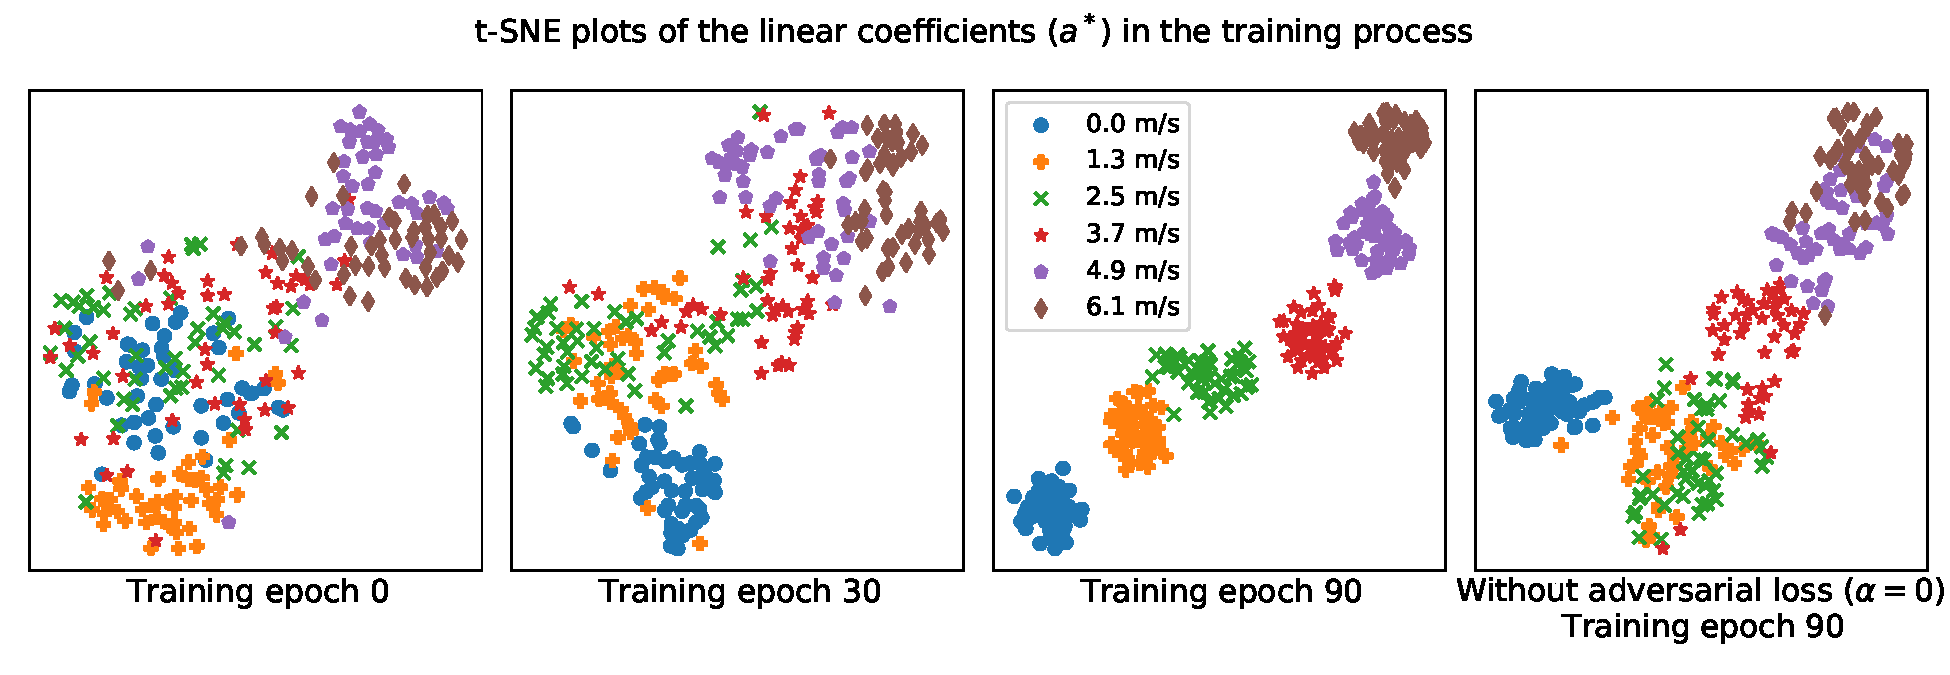
\includegraphics[width=1.0\linewidth]{figures/figure_training_tsne.pdf}
    \caption{\textbf{t-SNE plots showing the evolution of the linear weights ($a^*$) during the training process.} As the number of training epochs increases, the distribution of $a^*$ becomes more clustered with similar wind speed clusters near each other. The clustering also has a physical meaning: after training convergence, the right top part corresponds to a higher wind speed. This suggests that \DAML~successfully learned a basis function $\phi$ shared by all wind conditions, and the wind-dependent information is contained in the linear weights. Compared to the case without the adversarial regularization term (using $\alpha=0$ in Algorithm \ref{alg:DIML}), the learned result using our algorithm is also more explainable, in the sense that the linear coefficients in different conditions are more disentangled.}
    \label{fig:training-tsne}
\end{figure}

\subsection*{Offline Learning and Online Adaptive Control Development}
% Data collection procedure; there is a distribution shift in the data
\paragraph{Data Collection and Meta-Learning using \DAML} To learn an effective representation of the aerodynamic effects, we have a custom-built drone \rev{follow} a randomized trajectory for 2 minutes each in six different static wind conditions, with speeds ranging from \nowind~to \SI{22.0}{km/h}. \rev{However, in experiments we used wind speeds up to \highwind~(\highwindalt) to study how our methods extrapolate to unseen wind conditions (e.g., \cref{fig:error-wind-plot}).} The data is collected at \SI{50}{Hz} with a total of $36,000$ data points. \Cref{fig:training-data}(A) shows the data collection process, and Fig.~\ref{fig:training-data}(B) shows the inputs and labels of the training data, under one wind condition of \SI{13.3}{km/h}~(\SI{3.7}{m/s}). \Cref{fig:training-data}(C) shows the distributions of input data (pitch) and label data ($x-$component of the aerodynamic force) in different wind conditions. Clearly, a shift in wind conditions causes distribution shifts in both input domain and label domain, which motivates the algorithm design of \DAML. The same data collection process is repeated on the Intel Aero drone, \rev{to study whether the learned representation can generalize to a different drone.}

% daml algorithm is used to train representations of the wind  effects
On the collected datasets for both our custom drone and the Intel Aero drone, we apply the \DAML~algorithm to learn two representations $\phi$ of the wind effects. The learning process is done offline on a normal desktop computer, and depicted in \cref{fig:block-diagram}(B).
\Cref{fig:training-tsne} shows the evolution of the linear coefficients ($a^*$) during the learning process, where \DAML~learns a representation of the aerodynamic effects shared by all wind conditions, and the linear coefficient contains the wind-specific information. Moreover, the learned representation is explainable in the sense that the linear coefficients in different wind conditions are well disentangled (see \cref{fig:training-tsne}).
We refer to the ``\nameref{sec:methods}'' section for more details.

% Summary of all 5 control methods in results
\paragraph{Baselines and the Variants of Our Method} 
We briefly introduce three variants of our method and the \revision{three} baseline methods considered (details are provided in the ``\nameref{sec:methods}'' section). 
\revision{Each of the controllers is implemented in the position control loop and outputs a force command. The force command is fed into a kinematics block to determine a corresponding attitude and thrust, similar to \cite{mellinger_minimum_2011}, which is sent to the PX4 flight controller.}
\revision{The three baselines include: 
globally exponentially-stabilizing nonlinear tracking controller for quadrotor control
\cite{morgan_swarm_2015,shi2019neural,shi2018nonlinear},
incremental nonlinear dynamics inversion (INDI) linear acceleration control \cite{tal_accurate_2021}, and 
$\LOne$ adaptive control \cite{mallikarjunan_l1_2012,hanover_performance_2021}.
The primary difference between these baseline methods and \nf~is how the controller compensates for the unmodelled residual force (that is, each baseline method has the same control structure, in \cref{fig:block-diagram}(C), except for the estimation of the $\hat{f}$). In the case of the nonlinear baseline controller an integral term accumulates error to correct for the modeling error. The integral gain is limited by the stability \rev{of the interaction with the position and velocity error feedback} leading to slow model correction. In contrast, both INDI and $\LOne$ decouple the adaptation rate from the PD gains, which allow for fast adaptation. Instead, these methods are limited by more fundamental design factors, such as system delay, measurement noise, and controller rate.
}
% Both of the baseline methods include PID feedback and gravity compensation, while the nonlinear baseline also includes a feedforward term to account for the nominal dynamics model of the UAV (see the control diagram in \cref{fig:block-diagram}(C)). This control law generates a desired force required to track the desired trajectory. The desired force is fed into a kinematics block to determine the corresponding attitude and thrust to achieve that force (\cref{fig:block-diagram}(C)). 

Our method is illustrated in \cref{fig:block-diagram}(A,C) and replaces the integral feedback term with an adapted learning term. 
% REMOVED -> Our method also incorporates a first-order delay compensation block to account for attitude tracking and motor delay, which allows users to use a conventional regulation attitude controller. 
The deployment of our approach depends on the learned representation function $\phi$, and our primary method and two variants consider a different choice of $\phi$. \nf~is our primary method using a representation learned from the dataset collected by the custom-built drone, which is the same drone used in experiments. \revB{\nftransfer~uses the \nf~algorithm where the representation is trained} using the dataset collected by the aforementioned Intel Aero drone. \revB{\nfconstant~uses the online adaptation algorithm from \nf, but} the representation is an artificially designed constant mapping. \nftransfer~is included to show the generalizability and robustness of our approach with drone transfer, i.e., using a different drone in experiments than data collection. Finally, \nfconstant~demonstrates the benefit of using a better representation learned from the proposed meta-learning method \DAML. Note that \nfconstant~is a composite adaptation form of a Kalman-filter disturbance observer, that is a Kalman-filter \revision{augmented with} a tracking error update term.

% Define wind tasks, error metric, discuss data trimming
\subsection*{Trajectory Tracking Performance}
\revision{We quantitatively compare the performance of the aforementioned control methods when the UAV follows a \SI{2.5}{m} wide, \SI{1.5}{m} tall figure-8 trajectory with a lap time of \SI{6.28}{s} under constant, uniform wind speeds of \nowind, \lowwind~(\lowwindalt), \medwind~(\medwindalt), and \highwind~(\highwindalt) and under time-varying wind speeds of \sinwind~(\sinwindalt).}

\rev{
The flight trajectory for each of the experiments is shown in \cref{fig:trajectory}, which includes a warm up lap and six \SI{6.28}{s} laps. The nonlinear baseline integral term compensates for the mean model error within the first lap. As the wind speed increases, the aerodynamic force variation becomes larger and we notice a substantial performance degradation. INDI and $\LOne$ both improve over the nonlinear baseline, but INDI is more robust than $\LOne$ at high wind speeds. \nfconstant~outperforms INDI except during the two most challenging tasks: \highwind~and sinusoidal wind speeds. The learning based methods, \nf~and \nftransfer, outperform all other methods in all tests. \nf~outperforms \nftransfer~slightly, which is because the learned model was trained on data from the same drone and thus better matches the dynamics of the vehicle.
}

% Key quantitative performance comparisons from box plot and performance table
\rev{
In \cref{tab:flight-performance}, we tabulate the root-mean-square position error and mean position error values over the six laps for each experiment.
\Cref{fig:error-wind-plot} shows how the mean tracking error changes for each controller as the wind speed increases, and includes the standard deviation for the mean lap position error. In all cases, \nf~and \nftransfer~outperform the state-of-the-art baseline methods, including the \medwind, \highwind, and sinusoidal wind speeds all of which exceed the wind speed in the training data. %\nf~reports an average improvement of \SI{66}{\%} over the nonlinear baseline controller, \SI{35}{\%} over INDI, \SI{42}{\%} over $\LOne$, \SI{34}{\%} over \nfconstant, and \SI{12}{\%} over \nftransfer. Furthermore, \nf~and \nftransfer~outperform the other methods in the time-varying sinusoidal wind test, in \cref{tab:flight-performance}. 
}
All of these results presents a clear trend: adaptive control substantially outperforms the nonlinear baseline which relies on integral-control, and learning markedly improves adaptive control.
% which is very close to the localization uncertainty of the OptiTrack system (\SI{1}{cm}-\SI{2}{cm}, see more in the ``\nameref{sec:discussion}'' section). 

\begin{figure}[htbp]
    \centering
    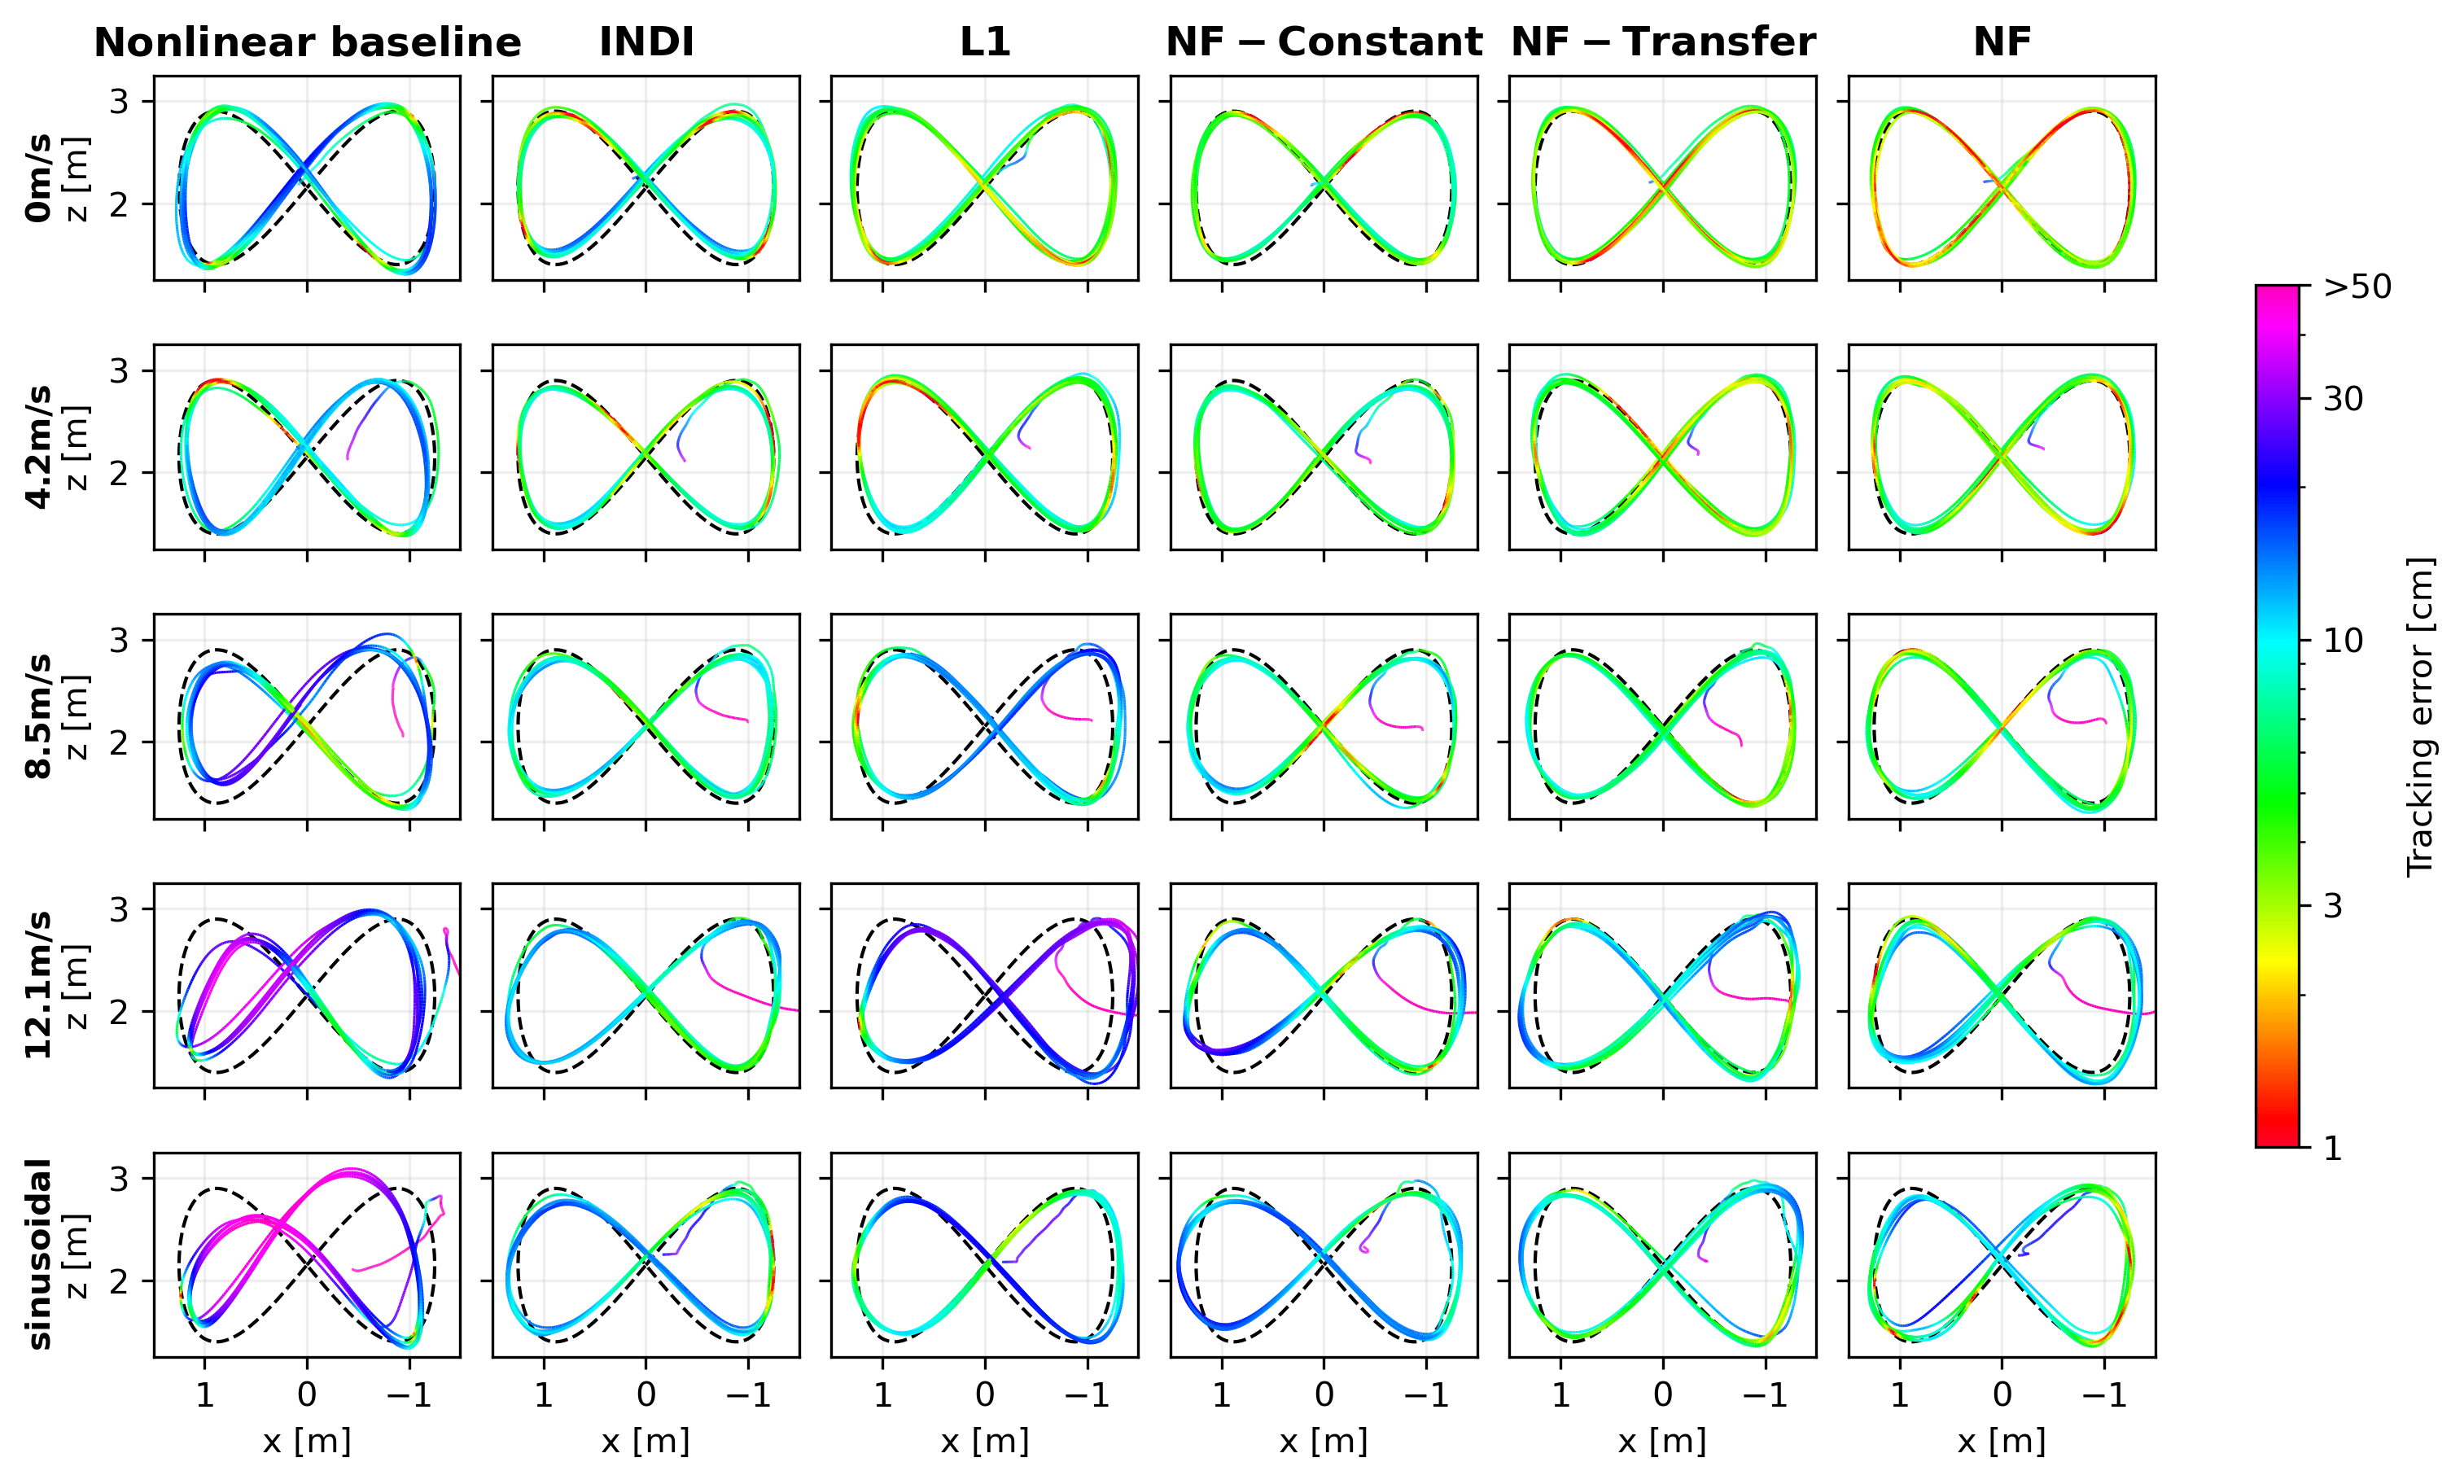
\includegraphics[width=0.97\linewidth]{figures/revision/trajectory-viz.png}
    \caption{
    \revision{
    \textbf{Depiction of the trajectory tracking performance of each controller in several wind conditions.} The baseline nonlinear controller can track the trajectory well, however, the performance \revB{substantially} degrades at higher wind speeds. INDI, $\LOne$, and \nfconstant~have similar performance and improve over the nonlinear baseline by estimating the aerodynamic disturbance force quickly. \nf~and \nftransfer~use a learned model of the aerodynamic effects and adapt the model in real time to achieve lower tracking error than the other methods.
    }}
    \label{fig:trajectory}
\end{figure}

% Motivation for precise flight control; flight through gate;
\subsection*{Agile Flight Through Narrow Gates}
Precise flight control in dynamic and strong wind conditions has many applications, such as rescue and search, delivery, and transportation. In this section, we present a challenging drone flight task in strong winds, where the drone must follow agile trajectories through narrow gates, which are only slightly wider than the drone. The overall result is depicted in \cref{fig:intro} and Video 1. As shown in \cref{fig:intro}(A), the gates used in our experiments are \SI{110}{cm} in width, which is only slightly wider than the drone (\SI{85}{cm} wide, \SI{75}{cm} long). To visualize the trajectory using long-exposure photography, our drone is deployed with four main light emitting diodes (LEDs) on its legs, where the two rear LEDs are red and the front two are white. There are also several small LEDs on the flight controller, the computer, and the motor controllers, which can be seen in the long-exposure shots. 


% overview of physical configuration of drone including its dimensions and LED locations
\paragraph{Task Design} 
% Define three tasks for experiments
We tested our method on three different tasks. In the first task (see \cref{fig:intro}(B,D,F-I) and Video 1), the desired trajectory is a \SI{3}{m} by \SI{1.5}{m} figure-8 in the $x-z$ plane with a lap time of \SI{5}{s}. A gate is placed at the left bottom part of the trajectory. The minimum clearance is about \SI{10}{cm} (see \cref{fig:intro}(I), which requires that the controller precisely tracks the trajectory. The maximum speed and acceleration of the desired trajectory are \SI{2.7}{m/s} and \SI{5.0}{m/s^2}, respectively. The wind speed is \SI{3.1}{m/s}. The second task (see Video 1) is the same as the first one, except that it uses a more challenging, time-varying wind condition, $3.1+1.8\sin(\frac{2\pi}{5}t)$\SI{}{m/s}. In the third task (see \cref{fig:intro}(C,E) and Video 1), the desired trajectory is a \SI{3}{m} by \SI{2.5}{m} ellipse in the $x-y$ plane with a lap time of \SI{5}{s}. We placed two gates on the left and right sides of the ellipse. As with the first task, the wind speed is \SI{3.1}{m/s}.

% Summary of image figure
\paragraph{Performance} For all three tasks, we used our primary method, \nf, where the representation is learned using the dataset collected by the custom-built drone. \Cref{fig:intro}(D,E) are two long-exposure photos with an exposure time of \SI{5}{s}, which is the same as the lap time of the desired trajectory. We see that our method precisely tracked the desired trajectories and flew safely through the gates (see Video 1). These long-exposure photos also captured the smoke visualization of the wind condition. We would like to emphasize that the drone is wider than the LED light region, since the LEDs are located on the legs (see \cref{fig:intro}(A)).  \Cref{fig:intro}(F-I) are four high-speed photos with a shutter speed of 1/200\SI{}{s}. These four photos captured the moment the drone passed through the gate in the first task, as well as the complex interaction between the drone and the wind. We see that the aerodynamic effects are complex and non-stationary and depend on the UAV attitude, the relative velocity, and aerodynamic interactions between the propellers and the wind.

\begin{figure} 
    \centering
    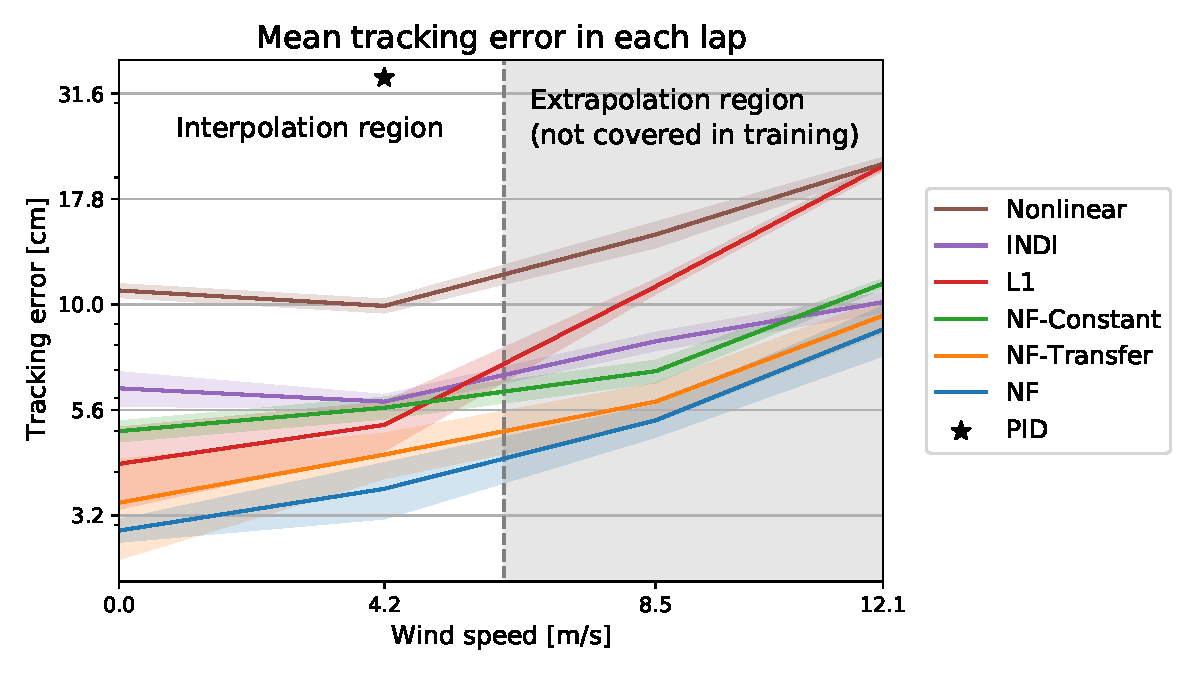
\includegraphics[width=0.8\linewidth]{figures/figure_error_windspeed.pdf}
    \caption{\revision{\textbf{Mean tracking errors of each lap in different wind conditions.} This figure shows position tracking errors of different methods as wind speed increases. Solid lines show the mean error over 6 laps and the shade areas show standard deviation of the mean error on each lap. The grey area indicates the extrapolation region, where the wind speeds are not covered in training. Our primary method (\nf) achieves state-of-the-art performance even with a strong wind disturbance.}}
    \label{fig:error-wind-plot}
\end{figure}

\begin{table}
\caption{\revision{Tracking error statistics in \SI{}{cm} for different wind conditions. Two metrics are considered: root-mean-square (RMS) and mean.}}
\label{tab:flight-performance}
\centering
\small
    \begin{tabular}{|c|cc|cc|cc|cc|cc|}
        \hline
        \multirow{3}{*}{\backslashbox{Method}{Wind speed\\ {[m/s]}}} & \multicolumn{2}{c|}{\multirow{2}{*}{0}}
        & \multicolumn{2}{c|}{\multirow{2}{*}{4.2}}
        & \multicolumn{2}{c|}{\multirow{2}{*}{8.5}}
        & \multicolumn{2}{c|}{\multirow{2}{*}{12.1}}
        & \multicolumn{2}{c|}{\multirow{2}{*}{$8.5+2.4\sin(t)$}} \\
        &&&&&&&&&&\\
        & RMS & Mean
        & RMS & Mean
        & RMS & Mean
        & RMS & Mean
        & RMS & Mean \\
        \hline
        
        \textbf{Nonlinear}
            &  11.9 &  10.8
            &  10.7 &  9.9
            &  16.3 &  14.7
            &  23.9 &  21.6
            &  31.2 &  28.2
        \\ \textbf{INDI}
            &  7.3 &  6.3
            &  6.4 &  5.9
            &  8.5 &  8.2
            &  10.7 &  10.1
            &  11.1 &  10.3
        \\ \textbf{L1}
            &  4.6 &  4.2
            &  5.8 &  5.2
            &  12.1 &  11.1
            &  22.7 &  21.3
            &  13.0 &  11.6
        \\ \textbf{NF-Constant}
            &  5.4 &  5.0
            &  6.1 &  5.7
            &  7.5 &  6.9
            &  12.7 &  11.2
            &  12.7 &  12.1
        \\ \textbf{NF-Transfer}
            &  3.7 &  3.4
            &  4.8 &  4.4
            &  6.2 &  5.9
            &  10.2 &  9.4
            &  8.8 &  8.0
        \\ \textbf{NF}
            &  \textbf{3.2} &  \textbf{2.9}
            &  \textbf{4.0} &  \textbf{3.7}
            &  \textbf{5.8} &  \textbf{5.3}
            &  \textbf{9.4} &  \textbf{8.7}
            &  \textbf{7.6} &  \textbf{6.9}
        \\ \hline
    \end{tabular}
\end{table}

\rev{\subsection*{Outdoor Experiments}
We tested our algorithm outdoors in gentle breeze conditions (wind speeds measured up to \SI{17}{km/h}). An onboard GPS receiver provided position information to the EKF, giving lower precision state estimation, and therefore less precise aerodynamic residual force estimation. Following the same aforementioned figure-8 trajectory, the controller reached \SI{7.5}{cm} mean tracking error, shown in \cref{fig:outdoor}.
}

% {\it
% The results should describe the experiments performed and the findings observed. The Results section should be divided into subsections to delineate different experimental themes. Subheadings should either be all phrases or all complete sentences. All data must be shown either in the main text or in the Supplementary Materials.

% For each result, discuss:

% 1. purpose/background of experiment

% 2. experimental approach

% 3. results

% 4. brief interpretation}